\documentclass[11pt,a4paper]{article}

\usepackage[utf8]{inputenc}
\usepackage[T1]{fontenc}
\usepackage[french]{babel}
\usepackage[margin=2.2cm]{geometry}
\usepackage{graphicx}
\usepackage{float}
\usepackage{xcolor}
\usepackage[hidelinks]{hyperref}

\setlength{\parindent}{0pt}
\setlength{\parskip}{6pt}

\begin{document}

% ===================== PAGE DE GARDE =====================
\begin{titlepage}
\centering
BUT Informatique -- 2e année\\
IUT de Maubeuge -- Université Polytechnique Hauts-de-France

\vspace{4cm}

{\Huge \textbf{SAÉ 3.01}}

\vspace{0.5cm}

{\LARGE Système de gestion scientifique\\d'un laboratoire de recherche}

\vspace{1cm}

{\Large Rapport provisoire -- fin du Sprint 1}

\vfill

\textbf{Équipe K.A.B.L}\\
Aïssa Ouameur -- Kieran Lelong -- Lucas Deudon -- Brahim Haddadi

\vspace{1cm}

14 octobre 2026
\end{titlepage}

\tableofcontents
\newpage

% ===================== 1. PLANIFICATION =====================
\section{Planification du projet}

\subsection{Contexte}

Le projet consiste à créer un site web pour un laboratoire de recherche d'environ 350 personnes. Le site permet de gérer l'organisation du laboratoire (départements, groupes, personnels), de déclarer les activités scientifiques et de faire des bilans sur une période.

Ce que le client nous a demandé lors de l'entretien du 2 septembre 2026 :
\begin{itemize}
  \item garder tout l'historique (on ne supprime jamais rien) ;
  \item chacun ne voit que ce qui le concerne (droits pyramidaux) ;
  \item une activité faite à plusieurs a un seul porteur, pour éviter les doublons ;
  \item la saisie doit être simple ;
  \item c'est le RH qui crée les comptes.
\end{itemize}

\subsection{Outils}

\begin{tabular}{|l|p{11cm}|}
\hline
\textbf{Outil} & \textbf{Utilisation} \\ \hline
Trello & Suivi du backlog et des sprints \\ \hline
GitHub & Partage du code, une branche par personne puis fusion dans main \\ \hline
PHP / PostgreSQL & Langage et base de données du site (sans JavaScript) \\ \hline
Supabase & Hébergement de la base de données \\ \hline
Alwaysdata & Hébergement du site \\ \hline
Moqups & Maquettes des pages \\ \hline
\end{tabular}

\subsection{Calendrier}

Nous sommes en alternance (FA), le projet se fait donc en 3 sprints.

\begin{tabular}{|l|l|l|l|}
\hline
\textbf{Sprint} & \textbf{Début} & \textbf{Revue} & \textbf{Temps en autonomie} \\ \hline
Sprint 0 & 02/09/2026 & 15/09/2026 & 9 h \\ \hline
Sprint 1 & 16/09/2026 & 13/10/2026 & 15 h \\ \hline
Sprint 2 & 14/10/2026 & 06/11/2026 & 18 h \\ \hline
Sprint 3 & 20/11/2026 & 06/01/2027 & 12 h \\ \hline
\end{tabular}

Le Sprint 0 a servi à comprendre le sujet, préparer l'entretien avec le client et écrire le backlog.

\subsection{Backlog}

Le projet est découpé en 16 user stories (US). Chaque US a une taille, convertie en story points (SP) :

\begin{tabular}{|c|c|c|c|}
\hline
\textbf{XS} & \textbf{S} & \textbf{M} & \textbf{L} \\ \hline
2 SP & 3 SP & 5 SP & 13 SP \\ \hline
\end{tabular}

\vspace{0.3cm}

\begin{tabular}{|c|p{9cm}|c|c|c|}
\hline
\textbf{US} & \textbf{Intitulé} & \textbf{Priorité} & \textbf{Taille} & \textbf{SP} \\ \hline
US-01 & Socle de données historisé & Must & L & 13 \\ \hline
US-02 & Identifier les personnels & Must & M & 5 \\ \hline
US-03 & Se connecter & Must & M & 5 \\ \hline
US-04 & Droits pyramidaux & Must & M & 5 \\ \hline
US-05 & Déléguer ses droits & Should & XS & 2 \\ \hline
US-06 & Déclarer une activité individuelle & Must & S & 3 \\ \hline
US-07 & Déclarer une activité collective & Must & M & 5 \\ \hline
US-08 & Confirmer sa participation & Must & S & 3 \\ \hline
US-09 & Rechercher, filtrer et trier ses activités & Must & XS & 2 \\ \hline
US-10 & Tableau de bord & Must & M & 5 \\ \hline
US-11 & Générer son rapport d'activités & Must & M & 5 \\ \hline
US-12 & Importer les enseignements (ICS) & Must & M & 5 \\ \hline
US-13 & Importer les publications (HAL) & Must & M & 5 \\ \hline
US-14 & Ouvrir une campagne de saisie & Must & S & 3 \\ \hline
US-15 & Geler les données d'une campagne & Should & S & 3 \\ \hline
US-16 & Rouvrir une campagne & Should & XS & 2 \\ \hline
\multicolumn{4}{|r|}{\textbf{Total}} & \textbf{71} \\ \hline
\end{tabular}

\subsection{Trello}

Chaque US est une carte Trello. Elle passe de la colonne \og Backlog \fg{} à \og Sprint \fg{}, puis \og En revue \fg{} et enfin \og Validé par le client \fg{}.

\begin{figure}[H]
\centering
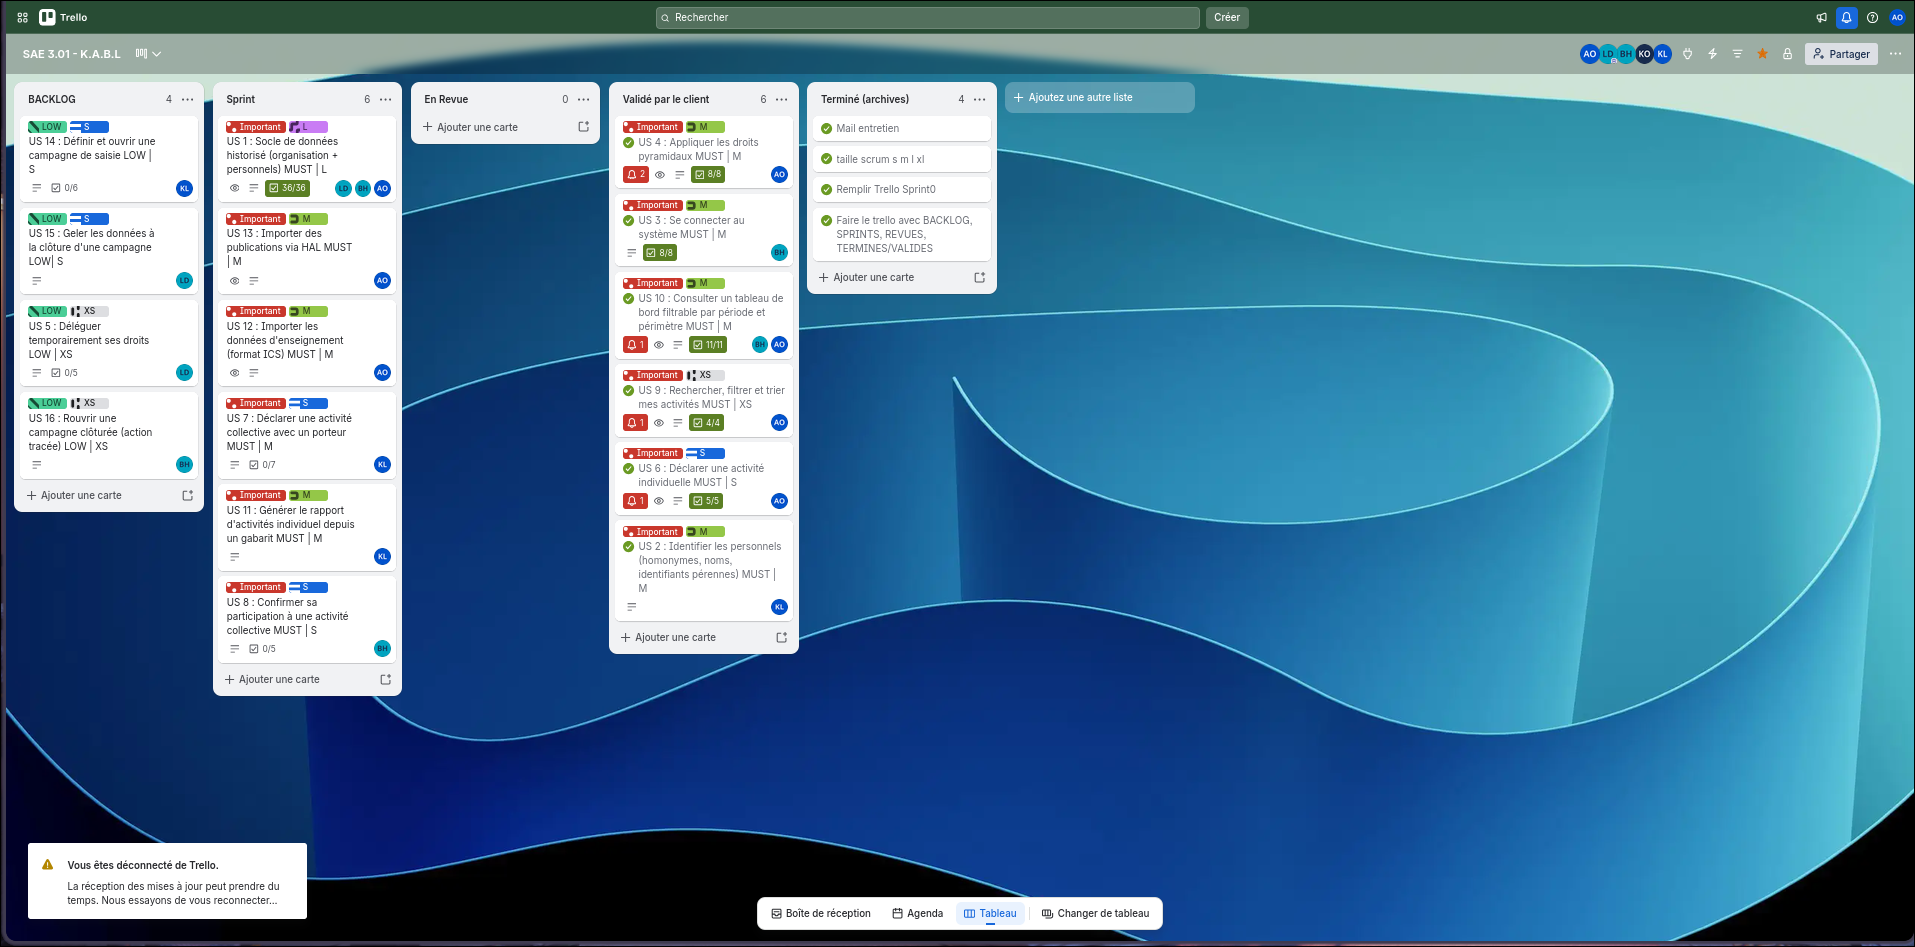
\includegraphics[width=\textwidth]{img/trello.png}
\caption{Notre Trello à la fin du Sprint 1}
\end{figure}

\newpage

% ===================== 2. UML ET NAVIGATION =====================
\section{UML et navigation}

\subsection{Diagramme de classes}

Chaque information qui change dans le temps a une date de début et une date de fin. Comme ça, on peut toujours savoir où était une personne à une date donnée.

\begin{figure}[H]
\centering
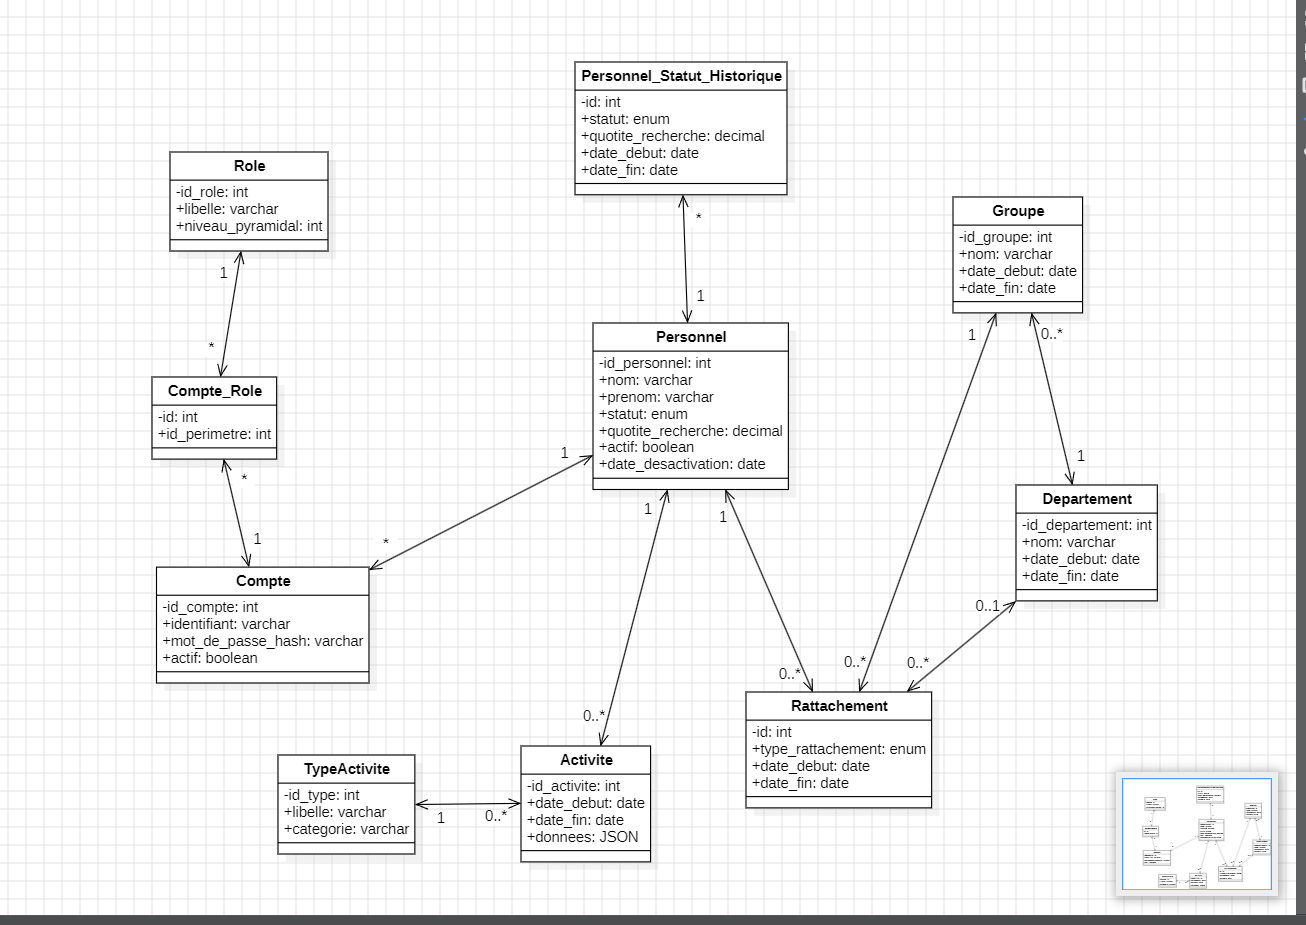
\includegraphics[width=\textwidth]{img/uml_conception.png}
\caption{Diagramme de classes}
\end{figure}

\colorbox{yellow}{\parbox{\dimexpr\textwidth-2\fboxsep}{
\textbf{Le diagramme va être modifié au Sprint 2}, car la base a évolué pendant le Sprint 1 :
\begin{itemize}
  \item le statut est déplacé dans une table d'historique ;
  \item ajout d'une table pour l'historique des noms ;
  \item ajout de deux tables pour les champs propres à chaque type d'activité ;
  \item suppression de la colonne JSON qui ne sert plus ;
  \item ajout des tables pour les activités collectives.
\end{itemize}
}}

\subsection{Les rôles}

Plus le niveau est petit, plus le rôle a de droits.

\begin{tabular}{|l|c|p{9cm}|}
\hline
\textbf{Rôle} & \textbf{Niveau} & \textbf{Ce qu'il voit} \\ \hline
Administrateur & 0 & Tout, et il gère les rôles \\ \hline
Directeur de laboratoire & 1 & Tout le laboratoire \\ \hline
Responsable de département & 2 & Son département \\ \hline
Responsable de groupe & 3 & Son groupe \\ \hline
Gestionnaire RH & 3 & Tout le laboratoire, sauf le contenu scientifique \\ \hline
Personnel & 4 & Seulement ses activités \\ \hline
\end{tabular}

\subsection{Navigation}

Ce schéma montre comment on passe d'une page à l'autre. Le menu change selon le rôle.

\begin{figure}[H]
\centering
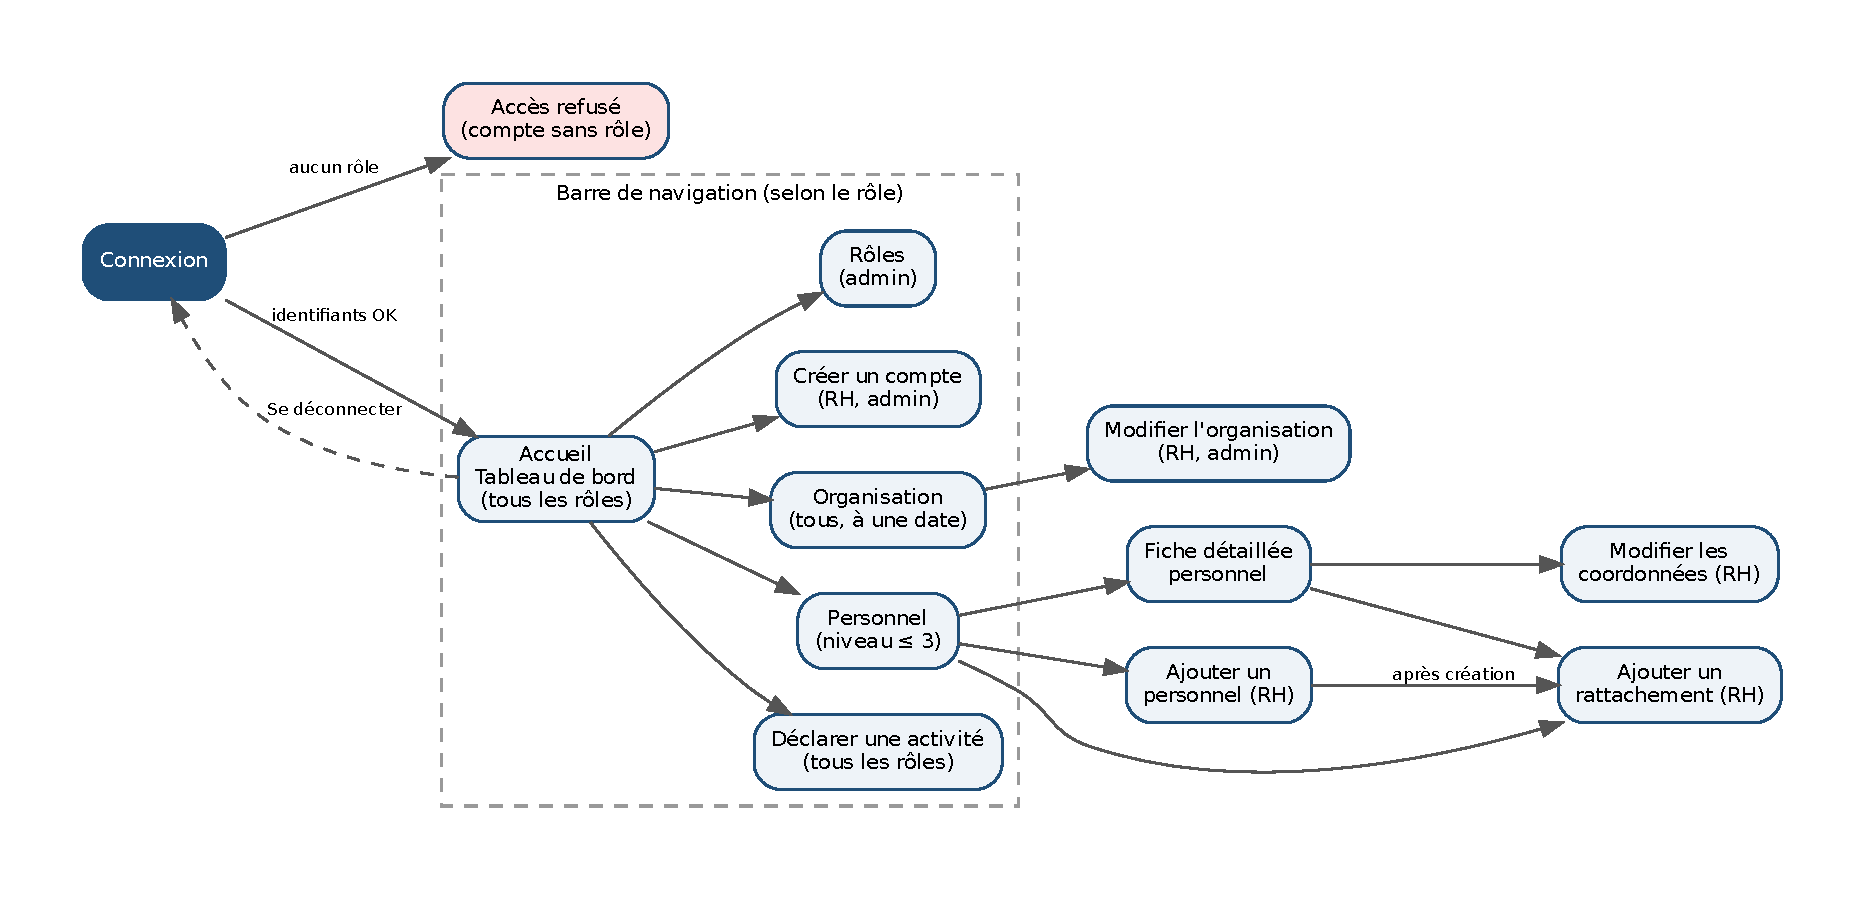
\includegraphics[width=\textwidth]{img/nav.pdf}
\caption{Navigation du site}
\end{figure}

\newpage

% ===================== 3. MAQUETTES =====================
\section{Maquettes}

\subsection{Maquettes Moqups}

Les pages ont été dessinées sur Moqups avant de coder :\\
\url{https://app.moqups.com/FCmUROPXbEEDy2K8OQC7VEABEoHTtDMf/view/page/a982d3ae6}

\colorbox{yellow}{\parbox{\dimexpr\textwidth-2\fboxsep}{
\textbf{À compléter :} ajouter les captures des maquettes Moqups.
}}

\subsection{Résultat}

Le site marche sur ordinateur, tablette et téléphone.

\begin{figure}[H]
\centering
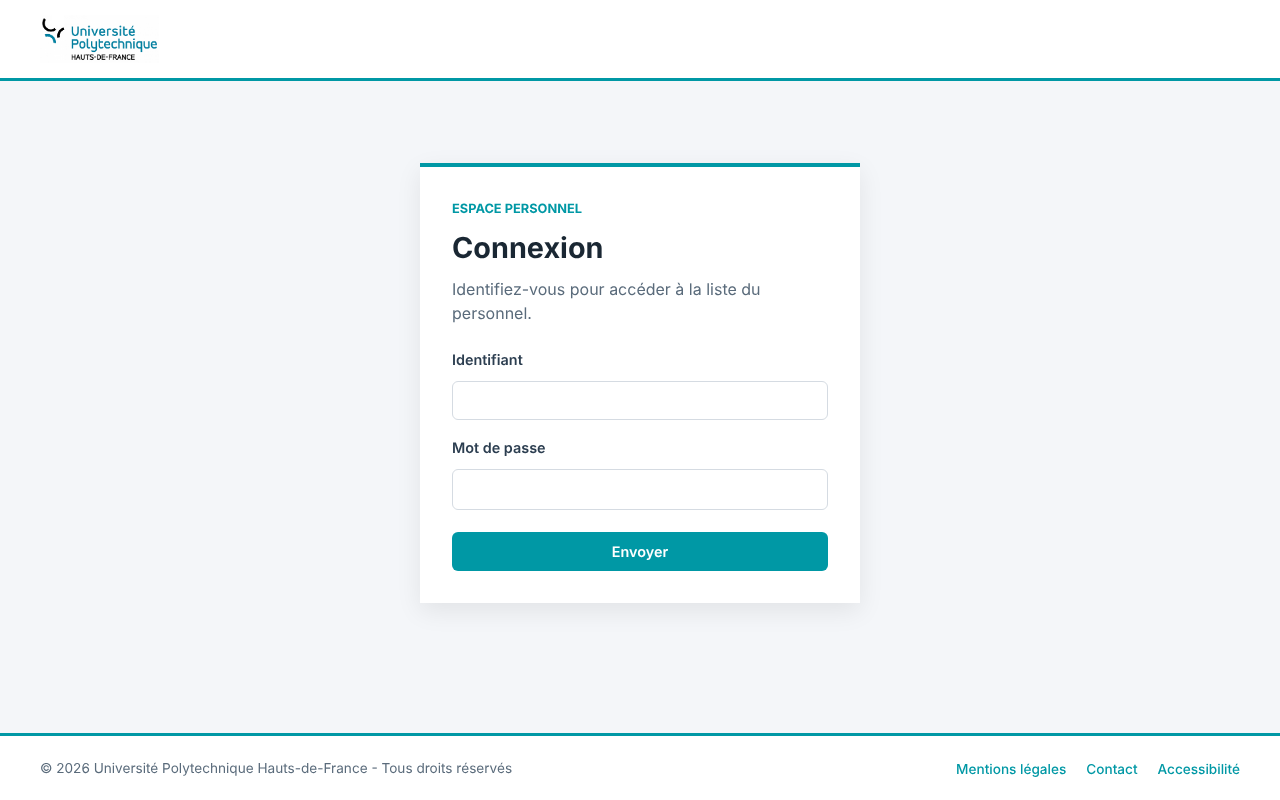
\includegraphics[width=0.8\textwidth]{img/connexion.png}
\caption{Page de connexion}
\end{figure}

\begin{figure}[H]
\centering
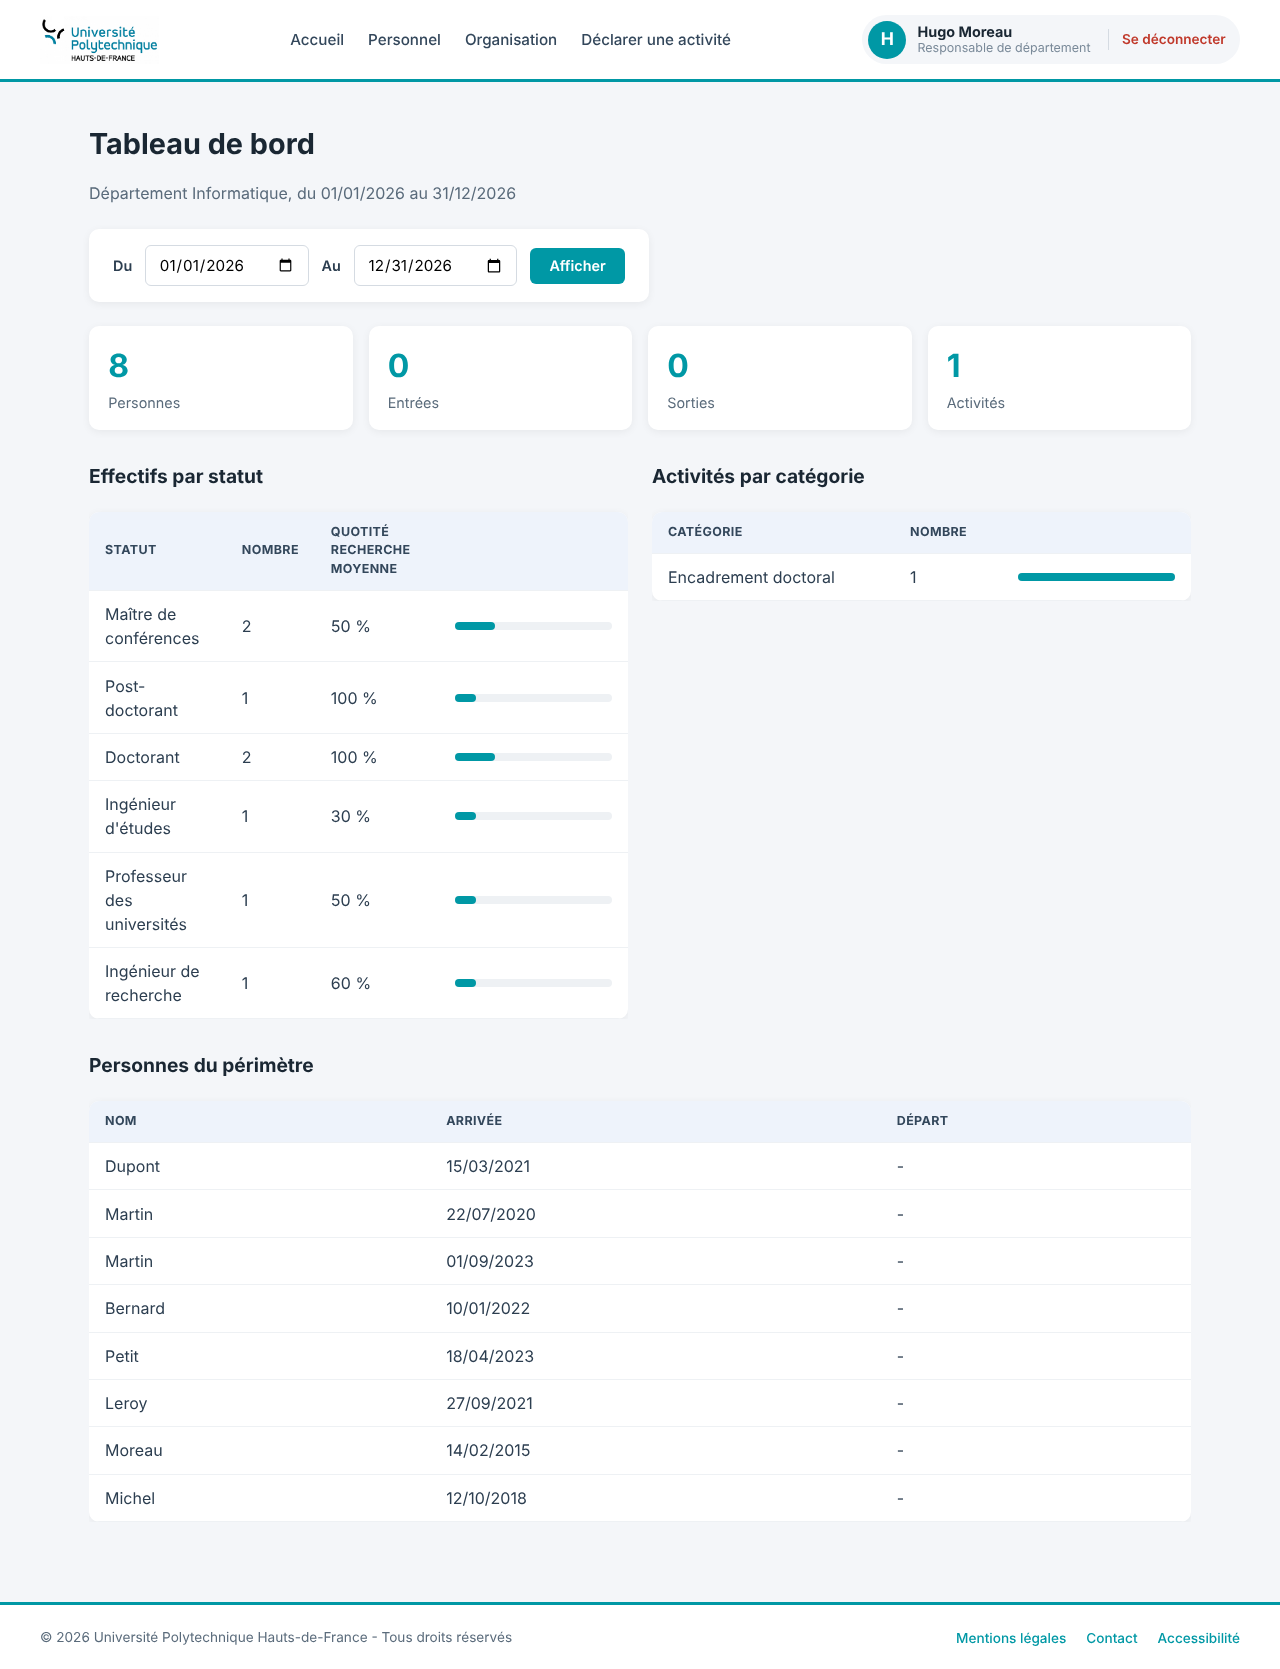
\includegraphics[width=0.8\textwidth,height=0.4\textheight,keepaspectratio]{img/tableau.png}
\caption{Tableau de bord}
\end{figure}

\begin{figure}[H]
\centering
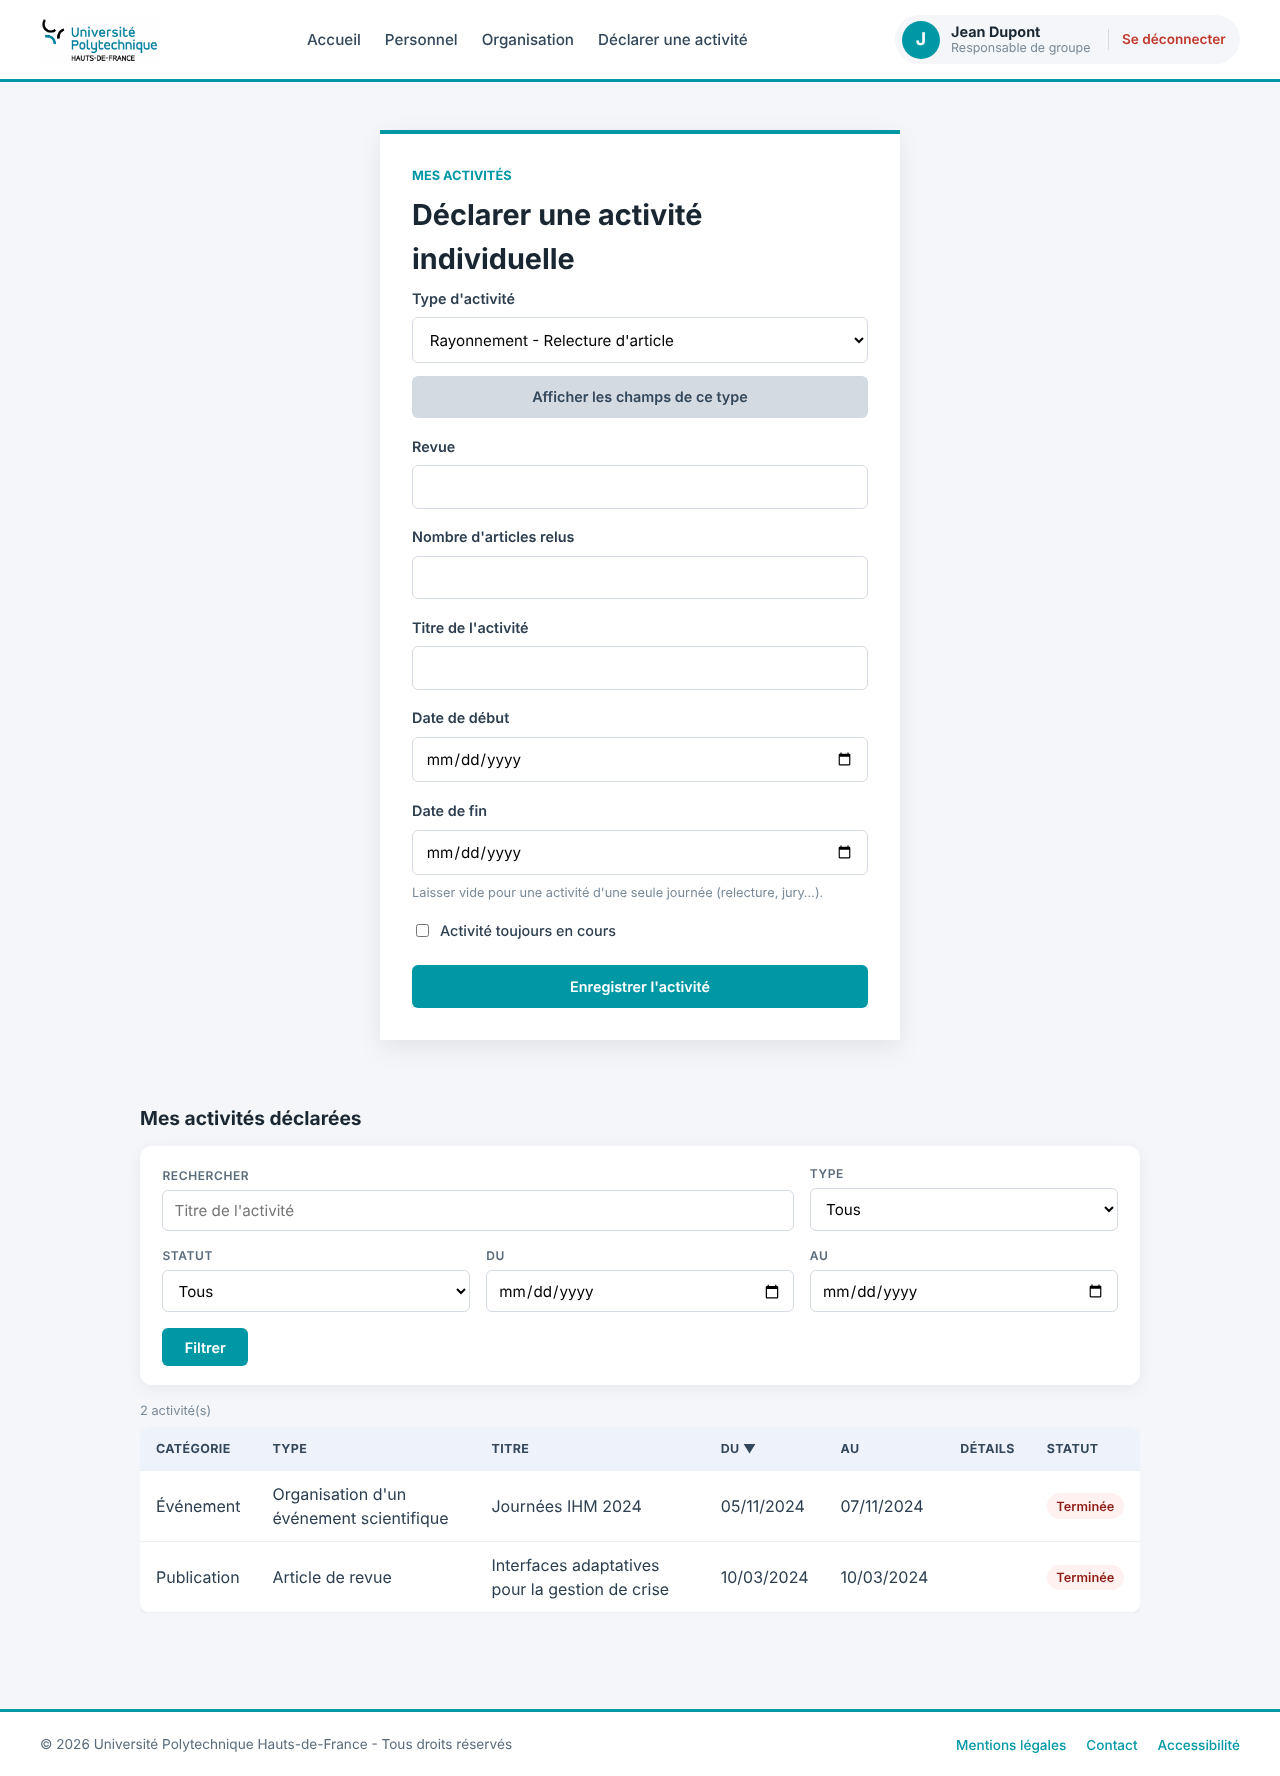
\includegraphics[width=0.8\textwidth,height=0.4\textheight,keepaspectratio]{img/declarer.png}
\caption{Déclarer une activité}
\end{figure}

\begin{figure}[H]
\centering
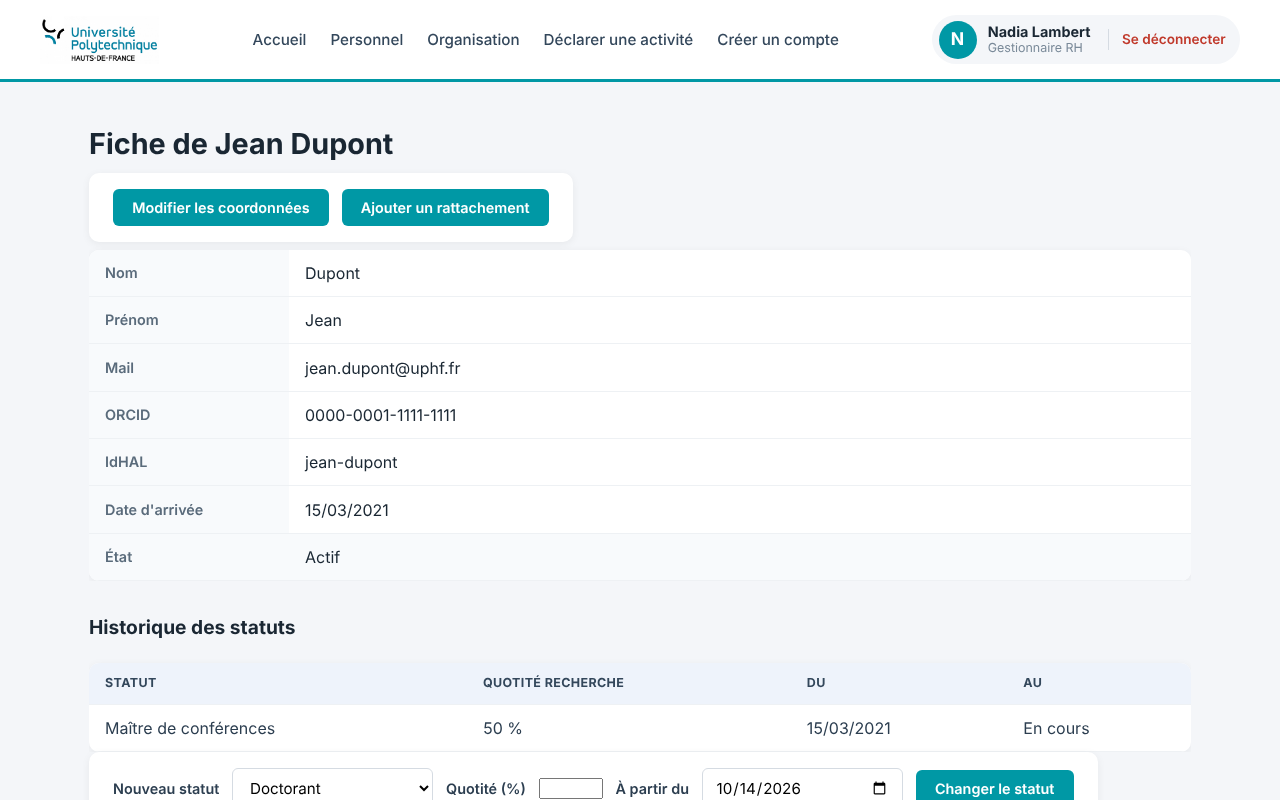
\includegraphics[width=0.8\textwidth]{img/fiche.png}
\caption{Fiche d'un personnel}
\end{figure}

\begin{figure}[H]
\centering
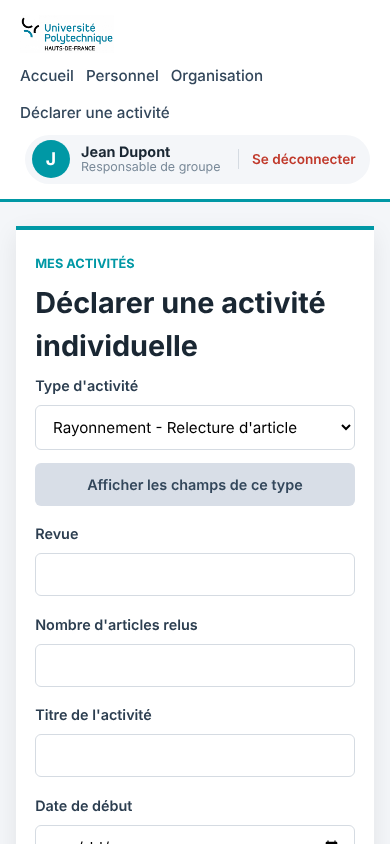
\includegraphics[height=7cm]{img/declarer_tel.png}
\hspace{1cm}
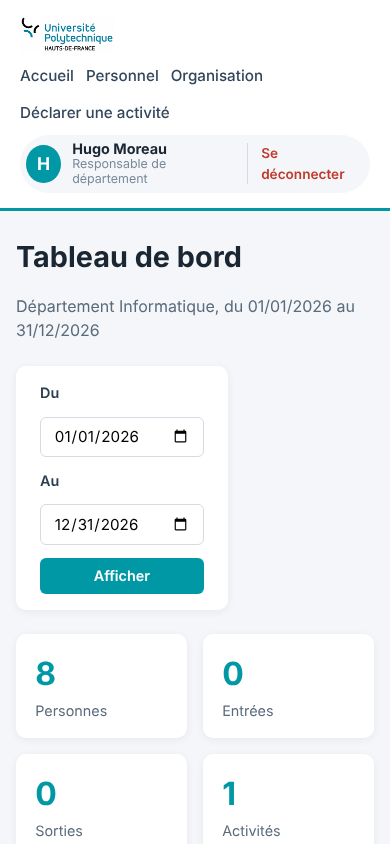
\includegraphics[height=7cm]{img/tableau_tel.png}
\caption{Version téléphone}
\end{figure}

\newpage

% ===================== 4. SPRINT 1 =====================
\section{Sprint 1}

\subsection{Objectif}

Permettre à un personnel de déclarer et de voir ses activités, avec l'historique et les droits.

\subsection{US du sprint}

\begin{tabular}{|c|p{6.5cm}|c|c|p{3.5cm}|}
\hline
\textbf{US} & \textbf{Intitulé} & \textbf{Taille} & \textbf{SP} & \textbf{Qui} \\ \hline
US-01 & Socle de données historisé & L & 13 & Lucas, Brahim, Aïssa \\ \hline
US-02 & Identifier les personnels & M & 5 & Kieran \\ \hline
US-03 & Se connecter & M & 5 & Brahim \\ \hline
US-04 & Droits pyramidaux & M & 5 & Aïssa \\ \hline
US-06 & Déclarer une activité & S & 3 & Aïssa \\ \hline
US-09 & Rechercher ses activités & XS & 2 & Aïssa \\ \hline
US-10 & Tableau de bord & M & 5 & Brahim, Aïssa \\ \hline
\multicolumn{3}{|r|}{\textbf{Total}} & \textbf{38} & \\ \hline
\end{tabular}

\subsection{Ce qu'on a fait}

\textbf{US-01 :} le RH crée les départements, les groupes et les personnels, les rattache, change leur statut, nomme les responsables et les désactive. Tout est daté.

\textbf{US-02 :} les homonymes sont différenciés, l'ancien nom est gardé, l'ORCID et l'IdHAL sont enregistrés.

\textbf{US-03 :} connexion avec un identifiant et un mot de passe.

\textbf{US-04 :} chacun ne voit que son périmètre. Le RH ne voit pas le contenu scientifique.

\textbf{US-06 :} on choisit un type d'activité et les bons champs s'affichent (par exemple \og Revue \fg{} pour une relecture).

\textbf{US-09 :} recherche, filtres et tri sur ses activités.

\textbf{US-10 :} tableau de bord avec les effectifs, les entrées et sorties, et un graphique des activités.

\newpage

% ===================== 5. REVIEW =====================
\section{Review du Sprint 1}

\subsection{Résultats}

\begin{tabular}{|c|p{7cm}|c|l|}
\hline
\textbf{US} & \textbf{Intitulé} & \textbf{SP} & \textbf{Résultat} \\ \hline
US-01 & Socle de données historisé & 13 & \colorbox{yellow}{\textbf{Partielle (bug)}} \\ \hline
US-02 & Identifier les personnels & 5 & Validée \\ \hline
US-03 & Se connecter & 5 & Validée \\ \hline
US-04 & Droits pyramidaux & 5 & Validée \\ \hline
US-06 & Déclarer une activité & 3 & Validée \\ \hline
US-09 & Rechercher ses activités & 2 & Validée \\ \hline
US-10 & Tableau de bord & 5 & Validée \\ \hline
\end{tabular}

\subsection{Le bug de l'US-01}

\colorbox{yellow}{\parbox{\dimexpr\textwidth-2\fboxsep}{
\textbf{Bug :} sur la page Organisation, une personne apparaît \textbf{responsable de groupe alors qu'elle n'est dans aucun groupe}. C'est impossible : un responsable de groupe est forcément dans son groupe.
}}

\begin{figure}[H]
\centering
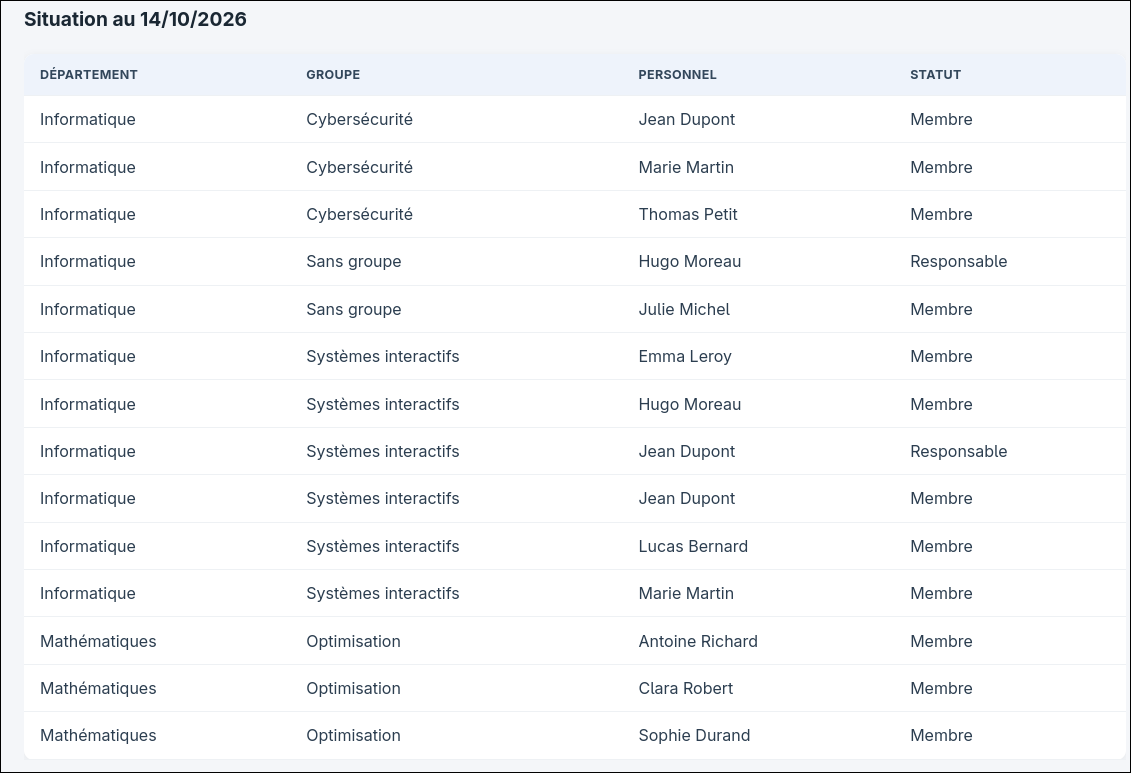
\includegraphics[width=0.8\textwidth]{img/bug_us01.png}
\caption{Hugo Moreau est \og Responsable \fg{} sur la ligne \og Sans groupe \fg{}}
\end{figure}

L'US-01 n'est pas comptée car elle n'est pas entièrement validée. Elle passe au Sprint 2.

\subsection{Ce qu'on ne peut pas encore tester}

\begin{itemize}
  \item \textbf{US-02 :} le rapprochement avec un import sera testé avec l'import HAL (US-13).
  \item \textbf{US-10 :} le comptage par porteur sera testé avec les activités collectives (US-07).
\end{itemize}

\subsection{Vélocité et burndown}

\begin{tabular}{|l|c|}
\hline
SP engagés & 38 \\ \hline
SP validés & 25 \\ \hline
Vélocité & 25 \\ \hline
SP restants & 46 \\ \hline
\end{tabular}

\begin{figure}[H]
\centering
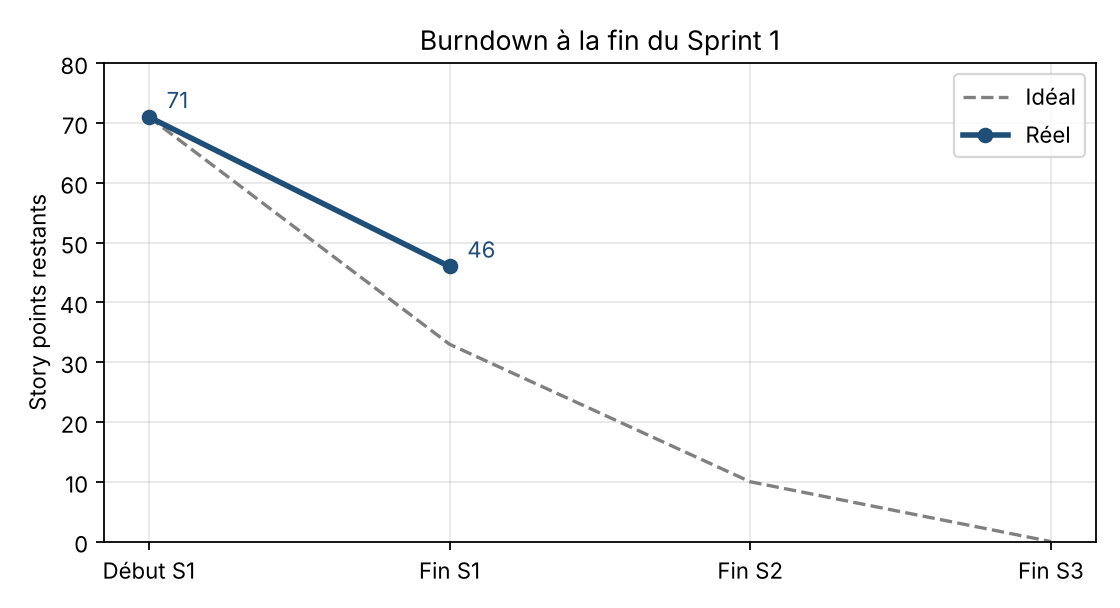
\includegraphics[width=0.75\textwidth]{img/burndown.png}
\caption{Burndown}
\end{figure}

On a 13 SP de retard sur le prévu, c'est l'US-01.

\begin{figure}[H]
\centering
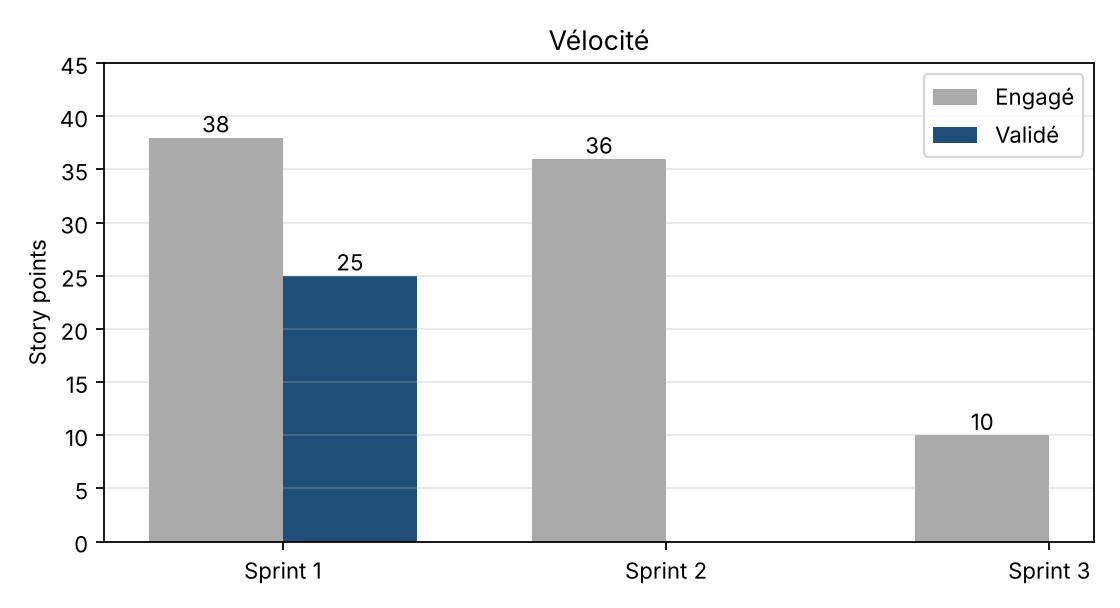
\includegraphics[width=0.75\textwidth]{img/velocite.png}
\caption{Vélocité}
\end{figure}

\subsection{Rétrospective}

\textbf{Ce qui a marché :}
\begin{itemize}
  \item 6 US sur 7 validées ;
  \item le site est en ligne.
\end{itemize}

\textbf{À améliorer :}
\begin{itemize}
  \item découper les grosses US ;
  \item faire valider les US pendant le sprint, pas à la fin ;
  \item garder l'UML à jour.
\end{itemize}

\newpage

% ===================== 6. SPRINT 2 =====================
\section{Planification du Sprint 2}

\subsection{Objectif}

Finir l'US-01, gérer les activités collectives, et faire les imports et l'export.

\subsection{US du sprint}

\begin{tabular}{|c|p{7.5cm}|c|c|p{2.8cm}|}
\hline
\textbf{US} & \textbf{Ce que c'est} & \textbf{Taille} & \textbf{SP} & \textbf{Qui} \\ \hline
US-01 & Corriger le bug et faire valider & L & 13 & Lucas, Brahim, Aïssa \\ \hline
US-07 & Activité faite à plusieurs, avec un seul porteur & M & 5 & Kieran \\ \hline
US-08 & Les participants confirment leur participation & S & 3 & Brahim \\ \hline
US-11 & Télécharger son rapport (Word ou CSV) & M & 5 & Kieran \\ \hline
US-12 & Importer les enseignements (.ics) & M & 5 & Aïssa \\ \hline
US-13 & Importer les publications depuis HAL & M & 5 & Aïssa \\ \hline
\multicolumn{3}{|r|}{\textbf{Total}} & \textbf{36} & \\ \hline
\end{tabular}

\subsection{Pourquoi 36 SP ?}

Notre vélocité est de 25. Mais l'US-01 est presque finie, il ne reste que le bug. Sans elle, il y a 23 SP de nouveau travail, ce qui est proche de notre vélocité.

\subsection{Ordre}

\begin{enumerate}
  \item Corriger l'US-01 en premier.
  \item Ajouter les nouvelles tables et mettre à jour l'UML.
  \item Faire les US-07, 11 et 12 en même temps.
  \item Finir par l'US-08 et l'US-13, qui ont besoin de l'US-07.
\end{enumerate}

\subsection{Sprint 3}

Il restera les US-05, 14, 15 et 16, soit 10 SP.

\end{document}
